%src/evExample.tex
%
\section{Discrete Example of \texorpdfstring{$E[g(x)]$}{E[g(x)]}, Equation \ref{EV}} %Appendix A
\begin{figure*}[b]
\begin{center}
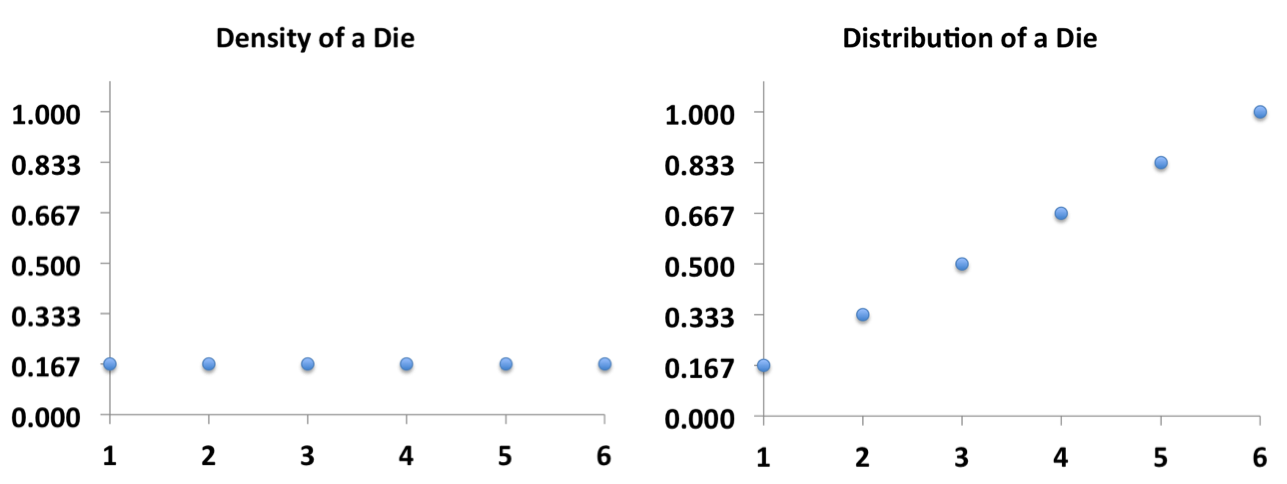
\includegraphics[width=0.8\linewidth]{figures/DieDenDist.png}
\end{center}
\caption{Density and distribution of a single die}
\end{figure*}
Assume our random variable $X$ is the result of rolling a single, fair 6-sided die.  
It's density and distribution are shown in Figure 3.
\begin{align*}
x    &= \text{The face value of rolling the die once} \\
x_i  &= \text{One of the specific (labeled) face values: 1, 2, 3, 4, 5, 6} \\
f(x) &= \text{The density function of $x$} \\
     &= \frac{1}{6} \\
g(x) &= \text{A function that produces a value given $x$} \\
     &= x \\
\shortintertext{The expected value (average) of rolling the die many times}
E[X] &= \sum_{i=1}^6 g(x_i)f(x_i) \\
     &= \frac{1}{6}\sum_{i=1}^6 g(x_i) \\
     &= \frac{1}{6}\left( 1 + 2 + 3 + 4 + 5 + 6\right) \\
     &= 3.5 \\
\shortintertext{Let's compute the expected value of the inverse of $X$} 
g_2(x) &= \frac{1}{x} \\
E\left[\frac{1}{X}\right] &= \sum_{i=1}^6 g_2(x_i)f(x_i) \\
                         &= \frac{1}{6}\sum_{i=1}^6 g_2(x_i) \\
                         &= \frac{1}{6}\left( \frac{1}{1} + \frac{1}{2} + \frac{1}{3} + \frac{1}{4} + \frac{1}{5} + \frac{1}{6}\right) \\
                         &= 0.408\overline{3} \\
\end{align*}
